% System components: what is shipped where. The editor extension carries no
% models; it pins the package, which carries the models and the engine.
\documentclass[tikz,border=6pt]{standalone}
% Shared preamble for all standalone paper figures.
% Palette and TikZ setup carried over from the legacy generator
% (paper/figures/scripts/build_paper_figures.py, TIKZ_HEADER) so the new
% figures keep the established visual identity.
\usepackage[T1]{fontenc}
\usepackage{amssymb}
\usepackage{helvet}
\renewcommand{\familydefault}{\sfdefault}
\usepackage{tikz}
\usepackage{pgfplots}
\pgfplotsset{compat=1.18}
\usetikzlibrary{arrows.meta,positioning,fit,calc,shapes.geometric}

\definecolor{mockblue}{HTML}{2E6F9E}
\definecolor{mockgreen}{HTML}{4F8A70}
\definecolor{mockred}{HTML}{C0392B}
\definecolor{mockgold}{HTML}{B08A2E}
\definecolor{mockgray}{HTML}{F4F1EC}
\definecolor{mockink}{HTML}{2B2B2B}

\tikzset{
  box/.style={draw=mockink!60, fill=white, rounded corners=2pt, align=center,
    inner sep=5pt, font=\small},
  main/.style={box, fill=mockgray, draw=mockink!70, thick},
  tzero/.style={box, fill=mockblue!14, draw=mockblue, thick},
  tone/.style={box, fill=mockgreen!14, draw=mockgreen, thick},
  ttwo/.style={box, fill=mockgold!16, draw=mockgold, thick},
  tthree/.style={box, fill=mockred!12, draw=mockred, thick},
  decision/.style={draw=mockink!70, fill=white, diamond, aspect=2.2,
    align=center, inner sep=2pt, font=\small},
  chip/.style={draw, rounded corners=4pt, inner sep=2.5pt, font=\scriptsize\bfseries,
    text=white},
  chipzero/.style={chip, fill=mockblue, draw=mockblue},
  chipone/.style={chip, fill=mockgreen, draw=mockgreen},
  chiptwo/.style={chip, fill=mockgold, draw=mockgold},
  chipthree/.style={chip, fill=mockred, draw=mockred},
  arrow/.style={-{Stealth[length=2.6mm]}, thick, mockink!80},
  yes/.style={arrow, mockgreen!80!black},
  no/.style={arrow, mockred!70!black},
  note/.style={font=\scriptsize, text=mockink!75, align=center},
  banner/.style={draw=mockink!70, fill=mockgray, rounded corners=3pt,
    align=center, inner sep=6pt, font=\small\bfseries},
}

\begin{document}
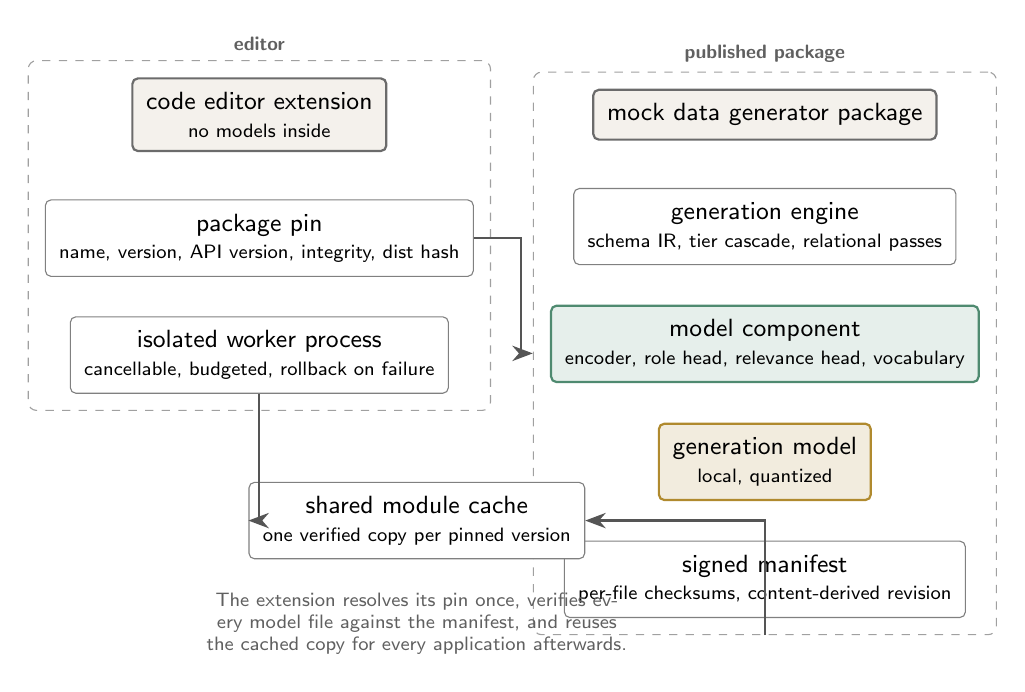
\begin{tikzpicture}[node distance=4mm]

% ---- editor side -----------------------------------------------------
\node[main] (editor) {code editor extension\\[-1pt]{\scriptsize no models inside}};
\node[box, below=6mm of editor] (pin) {package pin\\[-1pt]
  {\scriptsize name, version, API version, integrity, dist hash}};
\node[box, below=5mm of pin] (worker) {isolated worker process\\[-1pt]
  {\scriptsize cancellable, budgeted, rollback on failure}};
\node[draw=mockink!45, dashed, rounded corners=3pt, fit=(editor)(pin)(worker),
  inner sep=6pt, label={[font=\scriptsize\bfseries, text=mockink!75]above:editor}] (editorbox) {};

% ---- package side ----------------------------------------------------
\node[main, right=26mm of editor] (pkg) {mock data generator package};
\node[box, below=6mm of pkg] (engine) {generation engine\\[-1pt]
  {\scriptsize schema IR, tier cascade, relational passes}};
\node[tone, below=5mm of engine] (models) {model component\\[-1pt]
  {\scriptsize encoder, role head, relevance head, vocabulary}};
\node[ttwo, below=5mm of models] (llm) {generation model\\[-1pt]{\scriptsize local, quantized}};
\node[box, below=5mm of llm] (manifest) {signed manifest\\[-1pt]
  {\scriptsize per-file checksums, content-derived revision}};
\node[draw=mockink!45, dashed, rounded corners=3pt, fit=(pkg)(engine)(models)(llm)(manifest),
  inner sep=6pt, label={[font=\scriptsize\bfseries, text=mockink!75]above:published package}] (pkgbox) {};

% ---- cache -----------------------------------------------------------
\node[box, below=9mm of editorbox.south, xshift=20mm] (cache)
  {shared module cache\\[-1pt]{\scriptsize one verified copy per pinned version}};

\draw[arrow] (pin.east) -- ++(6mm,0) |- (pkgbox.west);
\draw[arrow] (pkgbox.south) |- (cache.east);
\draw[arrow] (worker.south) |- (cache.west);

\node[note, below=3mm of cache, text width=72mm]
  {The extension resolves its pin once, verifies every model file against the
   manifest, and reuses the cached copy for every application afterwards.};

\end{tikzpicture}
\end{document}
